\documentclass[aspectratio=169,10pt]{beamer}

\usetheme{Madrid}
\usecolortheme{default}
\setbeamertemplate{navigation symbols}{}
\setbeamertemplate{footline}[frame number]

\usepackage{amsmath,amssymb,booktabs,mathtools}
\usepackage{graphicx}
\usepackage{hyperref}

\definecolor{positive}{HTML}{0173B2}
\definecolor{negative}{HTML}{DE8F05}
\definecolor{emphasis}{HTML}{029E73}
\definecolor{neutral}{gray}{0.55}
\newcommand{\pos}[1]{\textcolor{positive}{#1}}
\newcommand{\con}[1]{\textcolor{negative}{#1}}
\newcommand{\HL}[1]{\textcolor{emphasis}{#1}}

\title{Stochastic Metal Enrichment in AuroraLF}
\subtitle{z=12.5 full UVLF and burst comparison}
\author{Presenter: Zhu Hourui}
\institute{AuroraLF}
\date{May 19, 2026}

\begin{document}

\begin{frame}
  \titlepage
\end{frame}

\begin{frame}{What changed}
\begin{columns}[T]
\column{0.50\textwidth}
\textbf{Existing UVLF path}
\begin{align*}
{\rm SFR}(t_i) &=
  \frac{f_b f_\star(M_{h,i}) \dot M_{h,i}}{10^9},\\
f_\star(M_h) &=
  \frac{2\epsilon_0}{(M_h/M_c)^{-\beta_\star}
  +(M_h/M_c)^{\gamma_\star}},\\
L_\nu &= L_{\nu,{\rm can}}+L_{\nu,{\rm TH}} .
\end{align*}
\column{0.46\textwidth}
\textbf{New diagnostic path}
\begin{itemize}
\item One-zone gas and metal reservoir on fixed MAH/SFR tracks.
\item Records gas metallicity and birth metallicity.
\item Birth metallicity gates top-heavy source-time SSP use.
\item No feedback into SFR, dust, or HMF weights.
\end{itemize}
\end{columns}
\end{frame}

\begin{frame}{IMF-gated UV convolution}
\begin{align*}
L_{\nu,{\rm can}}(t_{\rm obs}) &=
\int (1-I_{\rm TH})\,{\rm SFR}(t')\,
\ell_{\nu,{\rm can}}(t_{\rm obs}-t')\,dt',\\
L_{\nu,{\rm TH}}(t_{\rm obs}) &=
\int I_{\rm TH}\,{\rm SFR}(t')\,
\ell_{\nu,{\rm TH}}(t_{\rm obs}-t')\,dt'.
\end{align*}
\vspace{2mm}
\begin{columns}[T]
\column{0.48\textwidth}
\textbf{Mode definitions}
\begin{align*}
I_{\rm TH}&=0 \quad {\rm canonical},\\
I_Z&=\mathbf{1}[Z_{\rm birth}(t')\le0.05Z_\odot],\\
I_{\rm TH}&=\mathbf{1}[z(t')\ge z_{\rm TH}]I_Z,\\
I_{\rm TH}&=\mathbf{1}[z(t')\ge z_{\rm TH}]I_Z
\,\mathbf{1}\!\left[\frac{M_h}{\dot M_h}\le \tau_{\rm grow}\right].
\end{align*}
\column{0.44\textwidth}
\textbf{Run settings}
\begin{itemize}
\item $z_{\rm TH}=10$
\item $\tau_{\rm grow}=50~{\rm Myr}$
\item $Z_{\rm birth,TH}\le0.05Z_\odot$
\item top-heavy SSP metallicity $=0.05~Z_\odot$
\end{itemize}
\end{columns}
\end{frame}

\begin{frame}{One-zone metal update}
\small
\begin{align*}
M_{{\rm gas},i} &= f_{\rm gas}\,f_b\,M_{h,i},\\
Z_{{\rm birth},i}/Z_\odot &=
\frac{M_{Z,i-1}}{M_{{\rm gas},i}\,Z_\odot}
\,10^{\mathcal{N}(0,\sigma_{\rm birth})},\\
\Delta M_{\star,i} &= {\rm SFR}_i\,\Delta t_i\,10^9,\\
\eta_i &= \eta_0
\left(\frac{M_{h,i}}{M_\eta}\right)^{\alpha_\eta}
\left(\frac{1+z_i}{z_\eta}\right)^{\beta_\eta}
10^{\mathcal{N}(0,\sigma_\eta)},\\
y_i &= y\,\Bigl[1+(m_{\rm TH}-1)I_{{\rm TH},i}\Bigr]\,
10^{\mathcal{N}(0,\sigma_y)} .
\end{align*}
\begin{align*}
M_{Z,i}=\max\Bigl[
M_{Z,i-1}+Z_{\rm in}\Delta M_{{\rm in},i}
+y_i\Delta M_{\star,i}
-M_{Z,i-1}\bigl(1-e^{-[(1-R)+\eta_i]\Delta M_{\star,i}/M_{{\rm gas},i}}\bigr),
0\Bigr].
\end{align*}
\end{frame}

\begin{frame}{$z=12.5$ UVLF comparison}
\begin{center}
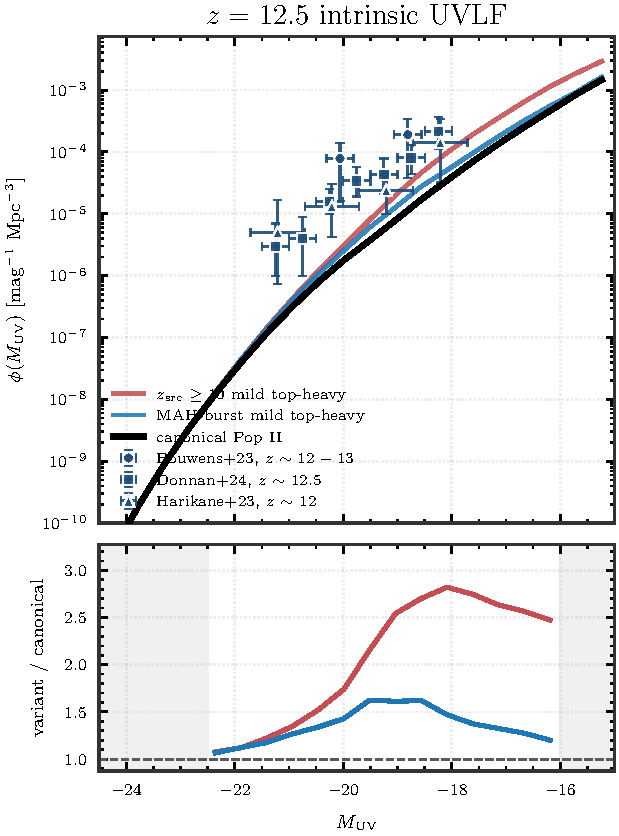
\includegraphics[height=0.82\textheight]{../assets/metallicity_z12p5_uvlf.pdf}
\end{center}
\end{frame}

\begin{frame}{Burst scatter model}
\begin{columns}[T]
\column{0.48\textwidth}
\textbf{Implemented perturbation}
\begin{align*}
{\rm SFR}_{\rm burst}(t_i)
&={\rm SFR}_{\rm smooth}(t_i)\,10^{\Delta_i},\\
\Delta_i &\sim
\mathcal{N}\!\left[-\frac{1}{2}\ln(10)\sigma_{\rm b}^2,
\sigma_{\rm b}\right].
\end{align*}
\begin{itemize}
\item Mean-preserving in linear SFR.
\item Piecewise correlated over $\tau_{\rm b}$.
\item Same burst realization across IMF modes.
\end{itemize}
\column{0.46\textwidth}
\textbf{$z=12.5$ test}
\begin{itemize}
\item $\sigma_{\rm b}=0.5~{\rm dex}$
\item $\tau_{\rm b}=20~{\rm Myr}$
\item seed $=777$
\item metallicity evolution uses burst SFR
\item UV convolution uses burst SFR
\end{itemize}
\end{columns}
\end{frame}

\begin{frame}{$z=12.5$ gate: delay and burst}
\begin{center}
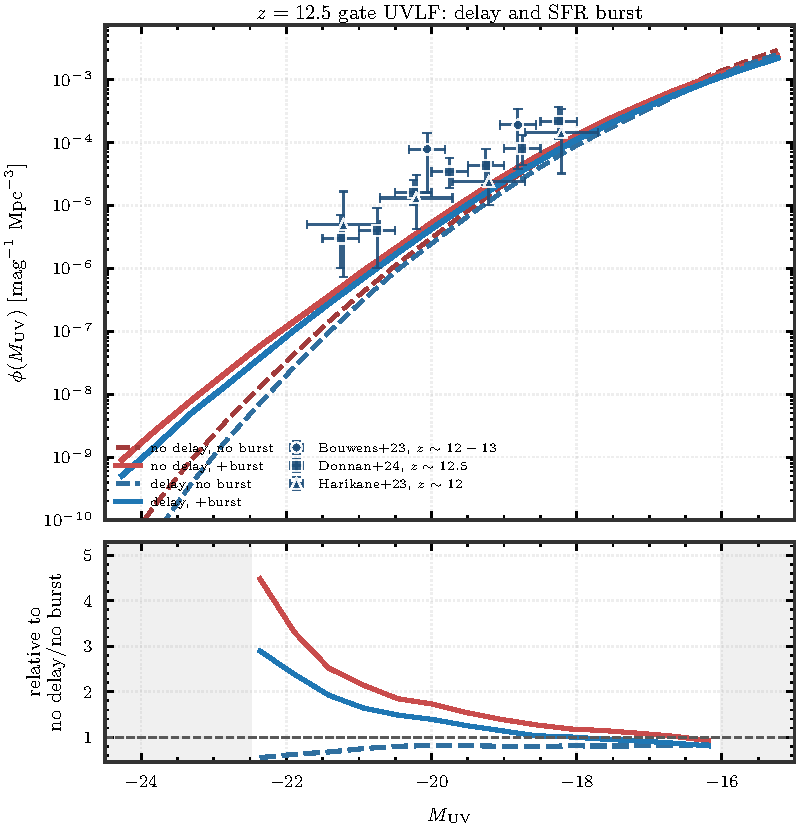
\includegraphics[height=0.82\textheight]{../assets/uvlf_gate_delay_burst_matrix_z12p5.pdf}
\end{center}
\end{frame}

\begin{frame}{$z=12.5$ run summary}
\begin{columns}[T]
\column{0.46\textwidth}
\textbf{Run}
\begin{itemize}
\item $N_{\rm mass}=3000$, $n_{\rm tracks}=1000$
\item HMF: Reed07 via \texttt{hmf}
\item stochastic metallicity enabled
\item $y=0.02$, $m_{\rm TH}=1.28$
\item $Z_{\rm birth,TH}\le0.05Z_\odot$
\end{itemize}
\column{0.50\textwidth}
\textbf{Result}
\begin{tabular}{lccc}
\toprule
Mode & UVLF ratio & $f_{\rm TH,src}$ & $Z_{\rm gas,final}$\\
\midrule
$z$-gate & 1.87 & 0.627 & 0.117\\
MAH-burst & 1.23 & 0.412 & 0.115\\
canonical & 1.00 & 0.000 & 0.114\\
\bottomrule
\end{tabular}

\vspace{2mm}
\small UVLF ratios are medians over model bins; metallicities are medians in $Z/Z_\odot$.
\end{columns}
\end{frame}

\begin{frame}{Burst run summary}
\begin{columns}[T]
\column{0.50\textwidth}
\textbf{Burst / no-burst UVLF}
\begin{tabular}{lccc}
\toprule
Mode & median & min & max\\
\midrule
canonical & 1.59 & 1.07 & 4.25\\
$z$-gate & 1.46 & 0.92 & 4.48\\
MAH-burst & 1.35 & 1.00 & 4.41\\
\bottomrule
\end{tabular}

\vspace{2mm}
\small Numbers use $-22.5\le M_{\rm UV}\le -16$.

\column{0.45\textwidth}
\textbf{Burst run IMF ratios}
\begin{tabular}{lcc}
\toprule
Mode & ratio & $f_{\rm TH,src}$\\
\midrule
$z$-gate & 1.80 & 0.669\\
MAH-burst & 1.16 & 0.440\\
canonical & 1.00 & 0.000\\
\bottomrule
\end{tabular}

\vspace{2mm}
\small Canonical $\phi$ median rises from $2.75\times10^{-6}$ to
$4.46\times10^{-6}$.
\end{columns}
\end{frame}

\begin{frame}{Delay and burst matrix}
\begin{columns}[T]
\column{0.48\textwidth}
\textbf{Gate UVLF, relative to no-delay/no-burst}
\begin{tabular}{lccc}
\toprule
Case & median & min & max\\
\midrule
no delay, +burst & 1.46 & 0.92 & 4.48\\
delay, no burst & 0.80 & 0.55 & 0.84\\
delay, +burst & 1.20 & 0.81 & 2.89\\
\bottomrule
\end{tabular}

\vspace{2mm}
\small Numbers use $-22.5\le M_{\rm UV}\le -16$.

\column{0.47\textwidth}
\textbf{Within-model effects}
\begin{tabular}{lc}
\toprule
Ratio & median\\
\midrule
delay +burst / delay no-burst & 1.48\\
delay +burst / no-delay +burst & 0.81\\
delay no-burst / no-delay no-burst & 0.80\\
\bottomrule
\end{tabular}

\vspace{2mm}
\small Delay suppresses the absolute gate UVLF; burst partly compensates but does not fully recover the no-delay burst case.
\end{columns}
\end{frame}

\begin{frame}{Interpretation}
\begin{itemize}
\item \HL{$z$-gate mode}: low-$Z$ gate leaves 62.7\% of source-times top-heavy.
\item In the observed magnitude range, $z$-gate boosts UVLF by $1.07$--$2.82$.
\item \HL{MAH-burst mode}: source fraction falls to 41.2\%; UVLF boost is only $1.07$--$1.62$.
\item Burst scatter brightens the UVLF; delay convolution suppresses it by $\simeq20\%$ in the observed range.
\item Even with low-$Z$ top-heavy SSPs and burst scatter, the model remains below many $z\simeq12.5$ points.
\end{itemize}
\end{frame}

\begin{frame}{References}
\small
\begin{thebibliography}{9}
\bibitem{reed2007} Reed et al. 2007, halo mass function fitting functions.
\bibitem{bpass} Eldridge et al. 2017, BPASS stellar population synthesis.
\bibitem{bpass221} Stanway \& Eldridge 2018, BPASS v2.2 binary populations.
\bibitem{auroralf} AuroraLF local implementation, \texttt{codex/topheavy-stochastic-metallicity}.
\end{thebibliography}
\end{frame}

\begin{frame}{Takeaway}
\begin{center}
\Large
The branch now tracks stochastic metal enrichment consistently with the same source-time top-heavy IMF gates used by the UVLF pipeline.

\vspace{4mm}
The burst branch adds short-timescale SFR scatter and shows that this helps the absolute UVLF more than the top-heavy relative ratio.
\end{center}
\end{frame}

\end{document}
